%%%%%%%%%%%%%%%%%%%%%%%%%%%%%%%%%%%%%%%%%%%%%%%%%%%%%%%%%%%%%%%%%%%%%%%%%%%%%%%%
\chapter{Introduction}\label{ch:intro}
%%%%%%%%%%%%%%%%%%%%%%%%%%%%%%%%%%%%%%%%%%%%%%%%%%%%%%%%%%%%%%%%%%%%%%%%%%%%%%%%
The recovery of the true structure of a scene captured by an image is 
arguably one of the core problems in Computer Vision. Although many properties
of a scene may be recovered, it is the geometry of the objects within the scene
that is of most use in many problems, as the geometry provides a strong model
from which to perform inference. In particular, the 3D shape of the underlying
objects is arguably the strongest cue for common tasks such as object
recognition and object localisation. However, the general problem or recovering
the 3D shape of an object from image (s) is incredibly ill-conditioned. Even when 
provided with multiple images, or additional information about the scene or
capturing conditions, 3D recovery is rife with ambiguities. As demonstrated
by~\cref{tbl:3d_recovery_methods}, many strategies have been proposed for
solving this problem. It is also important to note that there are two very
different outputs that can be obtained: \textit{dense shape} and 
\textit{sparse shape.} Sparse shape recovery has been
well studied in areas such as Structure-from-Motion where it has been
employed for large-scale reconstruction of urban scenes~\cite{agarwal2009building,torr1998robust}.
However, dense shape recovery is a much more difficult problem as the
complexity scales with the number of elements in the predicted
shape. In this thesis we consider only the problem of dense 3D shape recovery.

In contrast to the difficulty of the general case, the recovery of dense 3D
facial shape has been highly successful. Human faces have a number of qualities
that are desirable for shape recovery: they are extremely homogeneous in
configuration (all healthy human faces have two eyes, a nose and mouth in the
same approximate location), convex, exhibit approximately Lambertian 
reflectance~\cite{Sirovich:1987te,georghiades2001fromfew,Basri:2003ie,turk1991eigenfaces,Hallinan:1994dz,ramamoorthi2002analytic,ramamoorthi2001relationship,shashua1997photometric,moses1993face},
are largely captured from a single direction (frontal) and are deformable
but not self occluding. Furthermore, there exists a large amount of publicly
available imagery of faces and human faces are of significant interest to a 
number of fields including entertainment, medicine and psychology.
%%%%%%%%%%%%%%%%%%%%%%%%%%%%%%%%%%%%%%%%
\begin{table}[t]
	\centering
	\resizebox{\textwidth}{!}{%
		\begin{tabular}{@{}llccl@{}}
		\toprule
		\multicolumn{1}{c}{Classification}                  & \multicolumn{1}{c}{Method}                                                   & \# Images & Other Input                                                                       & \multicolumn{1}{c}{Output} \\ \midrule
		\multirow{4}{*}[-0.7cm]{Image Formation}            & Shape-from-Shading                                                           & $1$       & \begin{tabular}[c]{@{}c@{}}Reflectance Model, \\ Lighting Directions\end{tabular} & Surface Normals            \\ \cmidrule(l){3-5} 
		                                                    & \begin{tabular}[c]{@{}l@{}} (Un) Calibrated \\ Photometric Stereo\end{tabular} & $\geq 3$  & \begin{tabular}[c]{@{}c@{}}Lighting Directions \\ (If Calibrated)\end{tabular}    & Surface Normals            \\ \cmidrule(l){3-5} 
		                                                    & Shape-from-Contour                                                           & $1$       & Object Contour                                                                    & Coarse Surface Normals     \\ \cmidrule(l){3-5} 
		                                                    & Analysis-by-Synthesis                                                        & $1$       & 3D Model                                                                          & 3D Shape                   \\ \midrule
		\multicolumn{1}{c}{\multirow{2}{*}{Photogrammetry}} & Multi-View Stereo                                                            & $k$       & Camera Extrinsics                                                                 & 3D Shape                   \\ \cmidrule(l){3-5} 
		\multicolumn{1}{c}{}                                & Structure-from-Motion                                                        & $k$       & Corresponding Points                                                              & 3D Shape                   \\ \midrule
		\multicolumn{1}{c}{Other}                           & Shape Transfer                                                               & $1$       & 3D Model                                                                          & 3D or 2.5D Shape           \\ \bottomrule
		\end{tabular}
	}
	\caption{A summary of methods for recovering 3D shape from images. The two 
	         largest subcategories are image formation algorithms and 
	         photogrammetry.}
\label{tbl:3d_recovery_methods}
\end{table}
%%%%%%%%%%%%%%%%%%%%%%%%%%%%%%%%%%%%%%%%
An impressive example of the quality of 3D reconstruction possible is the
seminal work of \citet{RefWorks:96}. A commercial example of the
quality of reconstruction provided by a 3D Morphable Model (3DMM) method
is given in~\cref{fig:facegen_tom_hanks}. However, despite the success of 
3DMMs~\cite{RefWorks:96}, the problem of high quality 3D facial 
surface recovery from challenging images is still far from solved. For example,
the recovery of 3D facial surfaces under arbitrary conditions,
so called ``in-the-wild'' images, remains a challenging and active area of
research~\cite{KemelmacherShlizerman:2013iv,Suwajanakorn:2015gf,Suwajanakorn:2014bl,Snape:2015gl,roth2015unconstrained}.
In the case of 3DMMs, ``in-the-wild'' images present a significant challenge
as 3DMMs attempt to recover shape via an ``analysis-by-synthesis'' approach. An
``analysis-by-synthesis'' approach involves attempting to minimise the 
reconstruction error between the input image and a rendered output image that
is modelled via a set of parametric models and lighting conditions. Therefore,
in the case of ``in-the-wild'' facial images, ``analysis-by-synthesis'' is
incredibly challenging as an accurate result would require photo-realistic
rendering, which is currently not possible within the Computer Vision
literature. Moreover, the models employed contain a low number
of parameters and therefore have a tendency of being smooth and thus are not 
able to model fine details such as wrinkles.

Due to the insufficiencies of generic shape recovery, it is common to assume
that aspects of the scene are known a priory. In the case of the 3DMM, it is 
assumed that we know the class of object (e.g faces) and that we know the
approximate location of the face in the image. Knowing the class of object is
a strong but very powerful prior. This is most commonly exploited by introducing
some form of template or parametric model that describes the shape space of the
object class in question. However, there is a crucial problem that must be
solved before these shape priors can be employed. This is the problem of
\textit{correspondence}. For example, the 3DMM algorithm treats the entire
shape recovery problem as a correspondence problem. The 3D shape
model is used to synthesize an image which is then aligned by attempting to
minimise the reconstruction error of the rendered face against the input.
Another example is the seemingly unrelated area of Structure-from-Motion,
whereby a set of correspondences amongst a number of images is assumed. These
corresponding points are then factorized in order to recover both the underlying
3D shape and the parameters of the camera projection matrices that produced the
2D input points. In this case, the correspondence problem is assumed to have
already been solved. Therefore, when considering 3D facial shape recovery
methods it is also important to consider the problem of correspondence.
%%%%%%%%%%%%%%%%%%%%%%%%%%%%%%%%%%%%%%%%
\begin{figure}[t]
	\centering
	\hspace*{\fill}
	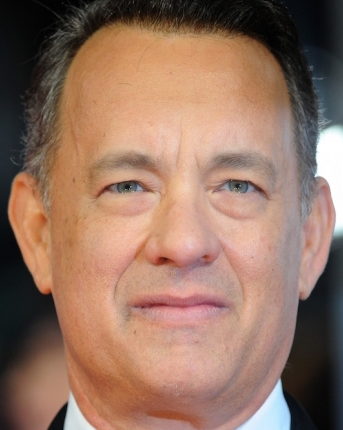
\includegraphics[height=1.8in]{introduction/images/tom_hanks_frontal_awards}\hfill
	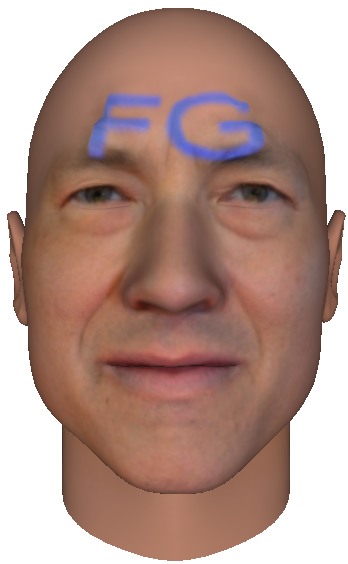
\includegraphics[height=1.8in]{introduction/images/tom_hanks_frontal_awards_facegen}\hfill
	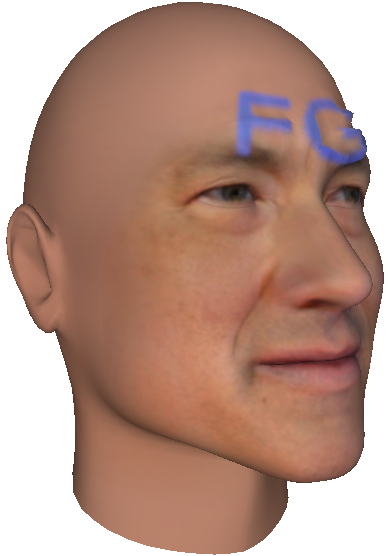
\includegraphics[height=1.8in]{introduction/images/tom_hanks_frontal_awards_facegen_profile}\hfill
	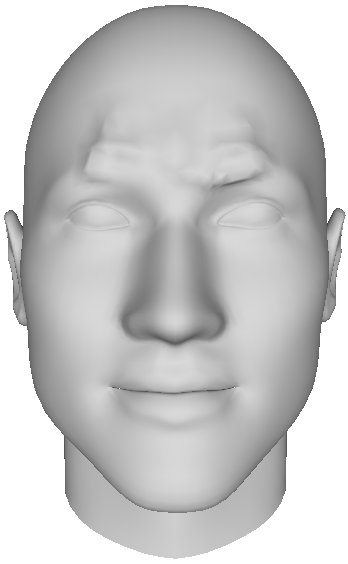
\includegraphics[height=1.8in]{introduction/images/tom_hanks_frontal_awards_facegen_no_texture}\hfill
	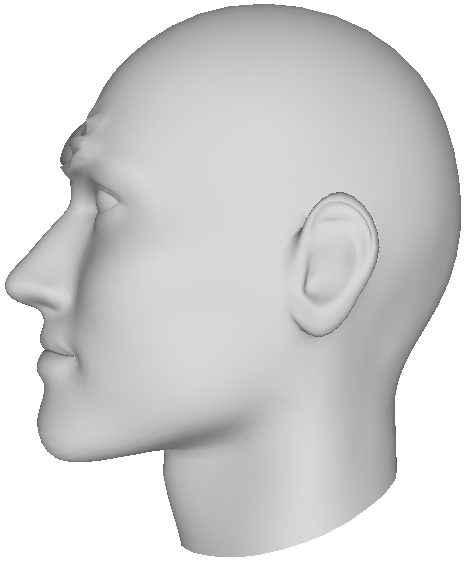
\includegraphics[height=1.8in]{introduction/images/tom_hanks_frontal_awards_facegen_no_texture_profile}
	\hspace*{\fill}
	\caption{An example of facial shape recovery by a 3D Morphable Model, 
	         provided by the commercial FaceGen software~\cite{facegen}. The
	         input image (leftmost) of Tom Hanks was provided and keypoints were
	         manually specified. Notice that the texture provides a strong 
	         likeness to Tom Hanks' face, yet the untextured mesh does not.}
\label{fig:facegen_tom_hanks}
\end{figure}
%%%%%%%%%%%%%%%%%%%%%%%%%%%%%%%%%%%%%%%%

In this thesis, we are interested in tackling the problem of 3D facial shape
recovery in challenging ``in-the-wild'' conditions. This is in contrast
to many works, such as the 3DMM, that focus on the recovery of facial shape
under ideal conditions (uniform frontal illumination, frontal face,
no expression, young Caucasian subject). As previously mentioned and summarised
in \cref{tbl:3d_recovery_methods}, there are 
a number of scenarios that may be considered in order to recover shape from
images. Given the breadth of possible scenarios, we have categorised them into
three major areas:
%%%%%%%%%%%%%%%%%%%%%%%%%%%%%%%%%%%%%%%%
\begin{itemize}
	\item \textbf{Single Image.} Given a single image, estimate the facial 
	      shape. This may involve employing template facial shapes, parametric
	      facial models or knowledge of the lighting conditions. 
	\item \textbf{Image Collections.} Given multiple images of faces, that may
	      or may not be of the same individual, estimate the facial shape for
	      each image. This may involve parametric models, employing illumination
	      constraints or known correspondences between the images.
	\item \textbf{Videos.} Given a sequence of images of a single individual,
	      recover their facial shape. This may involve known correspondences or
	      parametric models.
\end{itemize}
%%%%%%%%%%%%%%%%%%%%%%%%%%%%%%%%%%%%%%%%
Although there exists many other scenarios, these three provide methods of
recovery for the vast majority of media available for faces. In this thesis, we
chose to investigate a novel method for improving the state-of-the-art under
each of these three scenarios. The rest of this section will be devoted to
describing our contributions in the area of dense 3D facial shape recovery.
%%%%%%%%%%%%%%%%%%%%%%%%%%%%%%%%%%%%%%%%%%%%%%%%%%%%%%%%%%%%%%%%%%%%%%%%%%%%%%%%
\section{Contributions}\label{sec:intro_contrib}
%%%%%%%%%%%%%%%%%%%%%%%%%%%%%%%%%%%%%%%%%%%%%%%%%%%%%%%%%%%%%%%%%%%%%%%%%%%%%%%%
Given one or more images of faces, dense 3D facial shape recovery seeks to
predict the underlying 3D structure of the face (s) that produced the image (s).
The capturing conditions of these images largely determines the appropriateness
of a given technique. Many recovery methods make strong assumptions about
the capturing conditions, often assuming that the face has been captured in
a neutral expression under well-lit, stable conditions.
In this thesis, we approached the problem of 3D facial shape recovery under
challenging uncontrolled conditions using a variety of inputs and
assumptions, which are outlined below.

\textbf{Single Image Recovery: Statistical Models of Surface Normals.} Recovery
of 3D structure from single images remains the most challenging reconstruction
scenario. Without any data-based priors, the current state-of-the-art method
for single image shape recovery is the Shape-from-Shading (SfS) technique
of \citet{barron2015shape}. Despite being a very impressive example of the power
of generic priors, the reconstruction on objects such as faces is poor when 
compared to data-based face recovery methods. For this reason, it is common
to introduce data-based priors which restrict the recovery space to a specific
class of objects such as faces. Inspired by the success of SfS, we extend
the statistical surface normal models first introduced by 
\citet{smith2006recovering,smith2008facial} in the following ways:
%%%%%%%%%%%%%%%%%%%%%%%%%%%%%%%%%%%%%%%%
\begin{itemize}
	\item As noted by \citet{smith2006recovering,smith2008facial}, constructing
		  statistical models of surface normals is complicated by their
		  directional nature. However, we show that surface normals can be 
		  naturally embedded as kernels within statistical models. Unlike
		  the more complex embeddings proposed by~\cite{smith2006recovering,smith2008facial}, 
		  our kernel methods can be applied directly on normals. We also show
		  that the embeddings of~\cite{smith2006recovering,smith2008facial} 
		  can be presented as kernels.
    \item We extend the work of~\cite{smith2006recovering,smith2008facial}
          by proposing Kernel-PCA as a constraint in their Geometric-SfS 
          algorithm.
    \item Given the success of the image gradient in 2D image alignment~\cite{tzimiropoulos2011robust,cootes2001representing},
          we show that normals provide an effective feature representation
          for 2D image alignment of depth-based images. We show the natural
          robustness of normals to gross imaging defects such as occlusions
          by employing normals as a feature representation within a 
          Lucas-Kanade~\cite{lucas1981iterative,baker2004lucas}
          based parametric image alignment algorithm.
    \item Given the statistical model of surface normals and the Lucas-Kanade
          alignment algorithm, a natural extension is to use our statistical
          model of surface normals within the Active Appearance Model (AAM)~\cite{cootes2001active,matthews2004active} 
          algorithm. We demonstrate the effectiveness of our surface normal 
          Kernel-PCA for facial depth image alignment.
    \item We note that normals are analogous to gradients in the 3D image 
          domain. Therefore, we provide a proof of concept 3D Lucas-Kanade
          method that proposes two novel alignment algorithms. To the best of
          our knowledge, this is also the first comparative evaluation of
          extending state-of-the-art 2D Lucas-Kanade algorithms into the 3D
          image domain.
\end{itemize}
%%%%%%%%%%%%%%%%%%%%%%%%%%%%%%%%%%%%%%%%

\textbf{Image Collections: Class-Specific Photometric Stereo.} Photometric
Stereo (PS)~\cite{woodham1980photometric} takes as input 3 or more images of
a stationary object each lit by a unique, known point light source. 
By relaxing the need for known lighting directions, we arrive at the
Uncalibrated Photometric Stereo problem~\cite{hayakawa1994photometric,fan1997surface,yuille1999determining,basri2007photometric}.
Recently, \citet{KemelmacherShlizerman:2013iv} further relaxed the 
Uncalibrated PS algorithm to allow for recovery of spherical harmonics 
from a set of unrelated ``in-the-wild'' facial images. We formalise this
work~\cite{KemelmacherShlizerman:2013iv} in the following way:
%%%%%%%%%%%%%%%%%%%%%%%%%%%%%%%%%%%%%%%%
\begin{itemize}
	\item Provide a formal explanation for the ad hoc decomposition proposed
	      in \citet{KemelmacherShlizerman:2013iv}. Given this decomposition,
	      we show how it can be augmented with a robust low-rank matrix and 
	      sparse error term in order to better handle outliers in the input
	      images. We also investigate the use of a coarse but efficient
	      parametric alignment method based on sparse facial landmarking, 
	      in contrast to the more accurate but costly optical flow method 
	      proposed in~\cite{KemelmacherShlizerman:2013iv}.
\end{itemize}
%%%%%%%%%%%%%%%%%%%%%%%%%%%%%%%%%%%%%%%%

\textbf{Image Sequences: Face Flow.} Given a sequence of images (video) of
a single face, the recovery of a 3D surface using SfS constraints is
challenging. Although it is possible to recover surface normals
from video that contains sufficient lighting variation~\cite{brostow2011video,wenger2005performance,ma2007rapid,jones2011head}, these conditions are unlikely to be found within a typical
``in-the-wild'' video. Therefore, in order to recover 3D shape from videos,
we investigate a Structure-from-Motion (SfM) approach. The input to a 
Non-Rigid SfM algorithm is a set of correspondences across all input frames. 
Although these correspondences are typically sparse, dense SfM has recently been
successful~\cite{garg2013dense,newcombe2011dtam,agudo2014online,fragkiadaki2014grouping}.
However, the assumption of correspondences across all frames of a long 
``in-the-wild'' sequence is strong and difficult to satisfy in practise. 
Therefore, we propose the following:
%%%%%%%%%%%%%%%%%%%%%%%%%%%%%%%%%%%%%%%%
\begin{itemize}
	\item Typically, dense correspondences~\cite{Garrido:2014gn,agudo2014online} 
	      are acquired by optical flow~\cite{gibson1950perception,horn1981determining} 
	      algorithms. However, optical flow is very challenging in the general
	      case. Given we know the frames will contain faces, we propose to
	      impose a 2D facial motion prior on the optical flow fields. By
	      introducing a parametric motion model, the Lucas-Kanade~\cite{lucas1981iterative} 
	      algorithm allows the linearisation of the cost function and provides
	      extremely efficient alignment.
	      Furthermore, we augment the alignment method with a low-rank
	      constraint on the model coefficients that helps enforce a smoothness
	      prior across the length of the sequence.
	\item The training of the parametric motion model is the key constraint
	      on the performance of the above algorithm. Given the inability
	      of optical flow algorithms to correctly model the 3D motion field,
	      we opt to train our 2D flow field using an expressive 3D face model.
	      The face model is projected into the 2D plane and the flow fields
	      are learnt directly from these projections. This has a significant
	      advantage in that any alignment computed has a direct correspondence
	      with the 3D model used to compute the 2D motion field. Therefore,
	      approximate 3D shape is recovered directly from the 2D alignment.
\end{itemize}
%%%%%%%%%%%%%%%%%%%%%%%%%%%%%%%%%%%%%%%%
%%%%%%%%%%%%%%%%%%%%%%%%%%%%%%%%%%%%%%%%%%%%%%%%%%%%%%%%%%%%%%%%%%%%%%%%%%%%%%%%
\section{Publications}\label{sec:intro_pubs}
%%%%%%%%%%%%%%%%%%%%%%%%%%%%%%%%%%%%%%%%%%%%%%%%%%%%%%%%%%%%%%%%%%%%%%%%%%%%%%%%
In this section we provide a list of publications that were authored during the
course of this thesis. These publications are split into two sections, those
that are related to the contents of this thesis 
(\cref{subsec:intro_rel_pubs}) and other publications that 
are not directly relevant (\cref{subsec:intro_other_pubs}).
%%%%%%%%%%%%%%%%%%%%%%%%%%%%%%%%%%%%%%%%%%%%%%%%%%%%%%%%%%%%%%%%%%%%%%%%%%%%%%%%
\subsection{Related Publications}\label{subsec:intro_rel_pubs}
%%%%%%%%%%%%%%%%%%%%%%%%%%%%%%%%%%%%%%%%%%%%%%%%%%%%%%%%%%%%%%%%%%%%%%%%%%%%%%%%
%%%%%%%%%%%%%%%%%%%%%%%%%%%%%%%%%%%%%%%%
\begin{itemize}
	\item\bibentry{Snape:2014de}
	\item\bibentry{Snape:2015gl}
	\item\bibentry{Snape:2015hj}
\end{itemize}
%%%%%%%%%%%%%%%%%%%%%%%%%%%%%%%%%%%%%%%%
%%%%%%%%%%%%%%%%%%%%%%%%%%%%%%%%%%%%%%%%%%%%%%%%%%%%%%%%%%%%%%%%%%%%%%%%%%%%%%%%
\subsection{Other Publications}\label{subsec:intro_other_pubs}
%%%%%%%%%%%%%%%%%%%%%%%%%%%%%%%%%%%%%%%%%%%%%%%%%%%%%%%%%%%%%%%%%%%%%%%%%%%%%%%%
%%%%%%%%%%%%%%%%%%%%%%%%%%%%%%%%%%%%%%%%
\begin{itemize}
	\item\bibentry{menpo14}
	\item\bibentry{Chrysos:2015gt}
	\item\bibentry{trigeorgis2016mnemonic}
\end{itemize}
%%%%%%%%%%%%%%%%%%%%%%%%%%%%%%%%%%%%%%%%
The publications above are the joint work of the authors listed and do not
contain significant contributions to this thesis. Unless explicitly stated,
these publications are not considered to be my sole work.
%%%%%%%%%%%%%%%%%%%%%%%%%%%%%%%%%%%%%%%%%%%%%%%%%%%%%%%%%%%%%%%%%%%%%%%%%%%%%%%%
\section{Outline}\label{sec:introduction_outline}
%%%%%%%%%%%%%%%%%%%%%%%%%%%%%%%%%%%%%%%%%%%%%%%%%%%%%%%%%%%%%%%%%%%%%%%%%%%%%%%%
\cref{ch:background} provides a thorough literature review of existing
methodologies for 3D facial shape recovery. This includes relevant literature
for sparse and dense shape recovery, in order to provide a complete
picture as to the current state-of-the-art in 3D facial shape recovery.
\cref{ch:singl_imag} introduces contributions in the area of single image
facial shape recovery. A kernel method for representing surface normals is 
introduced and this kernel is used in a number of areas including 2D and 3D
image alignment and Shape-from-Shading.
\cref{ch:imag_coll} proposes a explicit algorithmic formulation for recovering
surface normals from unconstrained collections of facial images. This method,
dubbed Class-Specific Photometric Stereo, extends existing work on Uncalibrated
Photometric Stereo~\cite{KemelmacherShlizerman:2013iv,basri2007photometric}
with a robust method of recovering a per-image spherical harmonics.
\cref{ch:face_flow} considers the problem of dense facial correspondences. By
treating facial correspondence as a 2D image alignment problem, dense
correspondences between a parametric facial model and an image sequence are
computed. This model is easily extended to recover a 3D surface by leveraging
the correspondences between the image and a 3D model. 
Finally, \cref{ch:conclusions} summarises the findings of the previous chapters
and introduces possible areas of further research. 
%%%%%%%%%%%%%%%%%%%%%%%%%%%%%%%%%%%%%%%%%%%%%%%%%%%%%%%%%%%%%%%%%%%%%%%%%%%%%%%%